\documentclass[12pt,a4paper,ngerman]{article}
\usepackage{stylesheet}
\begin{document}
\TUHeader                          %  Bitte Ausfüllen!!!
%----------------------------
{Übung F: Übertragungsverhalten nachrichtentechnischer Systeme}                       %  Übungstitel
%----------------------------
{25.11.2014}                        %  Übungsdatum
%----------------------------
{05}                            %  Gruppen-Nr.
%----------------------------
{Thomas Neff}                   % Name des Protokollführers
%----------------------------
{
1.~Daniel Freßl, 1230028\\
2.~Thomas Neff, 1230319\\                    %  Übungsteilnehmer
3.~Thomas Pichler, 1230320 \\                   %  ...bei <4 Teilnehmer auskommentieren
4.~Martin Winter, 1130688\\
5.~Bernadette Schreyer, 1073076\\
}
%----------------------------
{Ao.Univ.-Prof. Dipl.-Ing. Dr. techn. Erich Leitgeb}
{Max Henkel}                          %  Betreuer
%----------------------------
{Graz}                              %  Ort der Protokollerstellung
{\today}                            %  Datum Protokollerstellung




\pagebreak
  
\tableofcontents
  
\pagebreak

%-------------------------------------------------------------------------------
%
% Beginn des Protokolls
%
%-------------------------------------------------------------------------------

\section{Demodulation eines QPSK-Signals mit unbekannten Paramteren}
\subsection{Aufgabenstellung}
Gegeben ist ein Signal, welches mittels QPSK auf einen HF-Träger moduliert wurde. Sie sollen dieses Signal nun mit dem in der Software integrierten digitalen Demodulator demodulieren. Da Ihnen die Paramter Trägerfrequenz, Symbolrate und senderseitig verwendetes Filter unbekannt sind, müssen Sie diese bestimmen.
\begin{itemize}
\item Bestimmen Sie die Trägerfrequenz und stellen Sie das Signal in Frequenz- und Zeitbereich sinnvoll dar. 
\item Bestimmen Sie die Symbolrate. Versuchen Sie dazu die Darstellung des Spektrums zu glätten.
\item Bestimmen Sie anhand des Spektrums den Filtertyp und dessen Parameter.
\item Demodulieren Sie das Signal. Stellen Sie Konstellations- und Augendiagramm sowie das Spektrum des Signals dar. 
\item Woran ist erkennbar, dass der richtige Filtertyp gefunden wurde. Überprüfen Sie ihre Antwort durch Veränderung der Einstellungen
\end{itemize}
\subsection{Messaufbau}
Das zu analysierende Signal wurde mit einem Vektorsignalgenerator generiert und mit dem Oszilloskop für die Analyse digitalisiert.  
\subsection{Tabellen}
Es waren keine Tabellen aufzunehmen. 
\subsection{Formeln}
Die Formel für die Nyquist-Frequenz lautet
\begin{equation}
f_N = \frac{f_S}{2}
\end{equation}
Die absolute Bandbreite ergibt sich durch
\begin{equation}
B = B_N (1+\alpha)
\end{equation}
\subsection{Berechnungsbeispiele}

\subsection{Diagramme}
\begin{figure}[H]
\centering
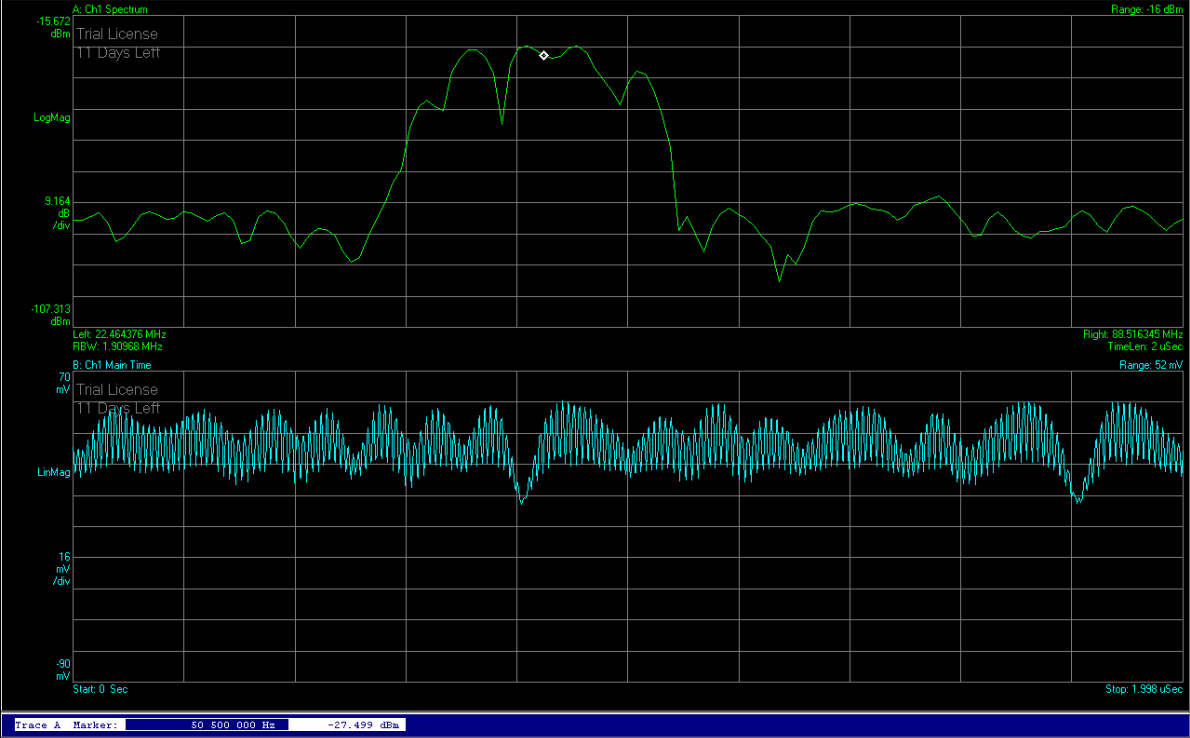
\includegraphics[width=\textwidth]{figures/Aufgabe1_QPSK.jpg} 
\caption{Test}
\end{figure}

\begin{figure}[H]
\centering
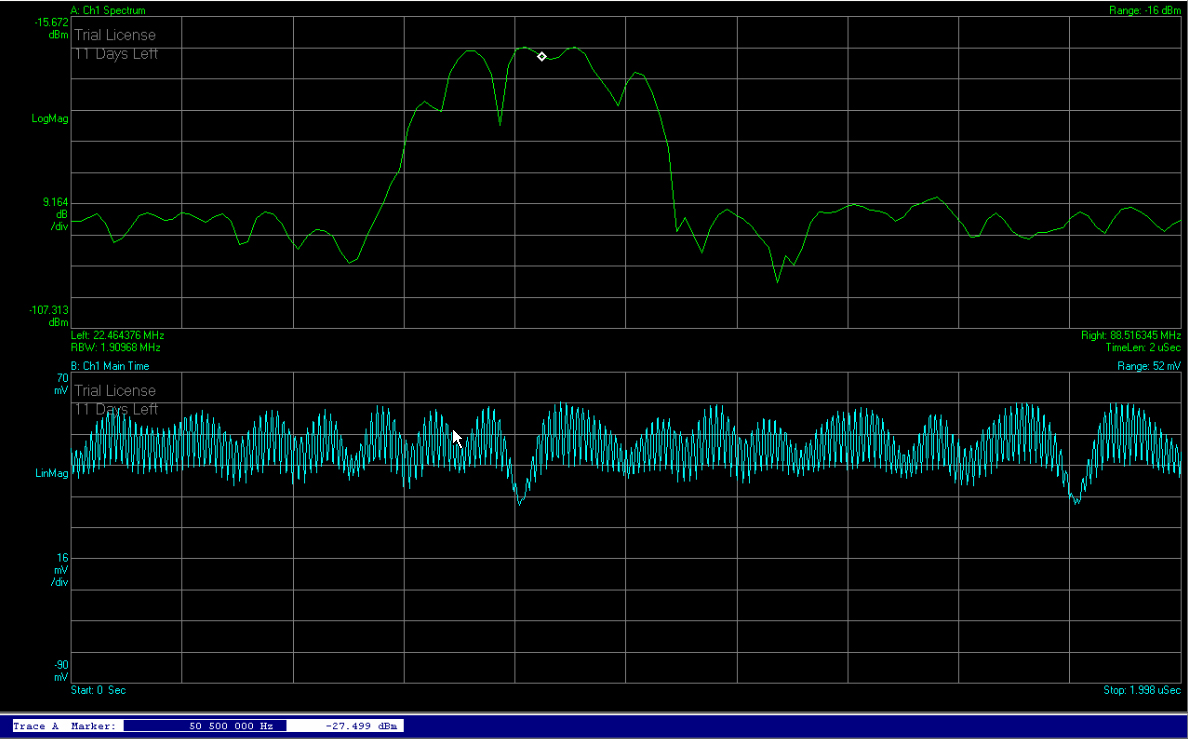
\includegraphics[width=\textwidth]{figures/Aufgabe1_QPSK_.jpg} 
\caption{Test}
\end{figure}

\begin{figure}[H]
\centering
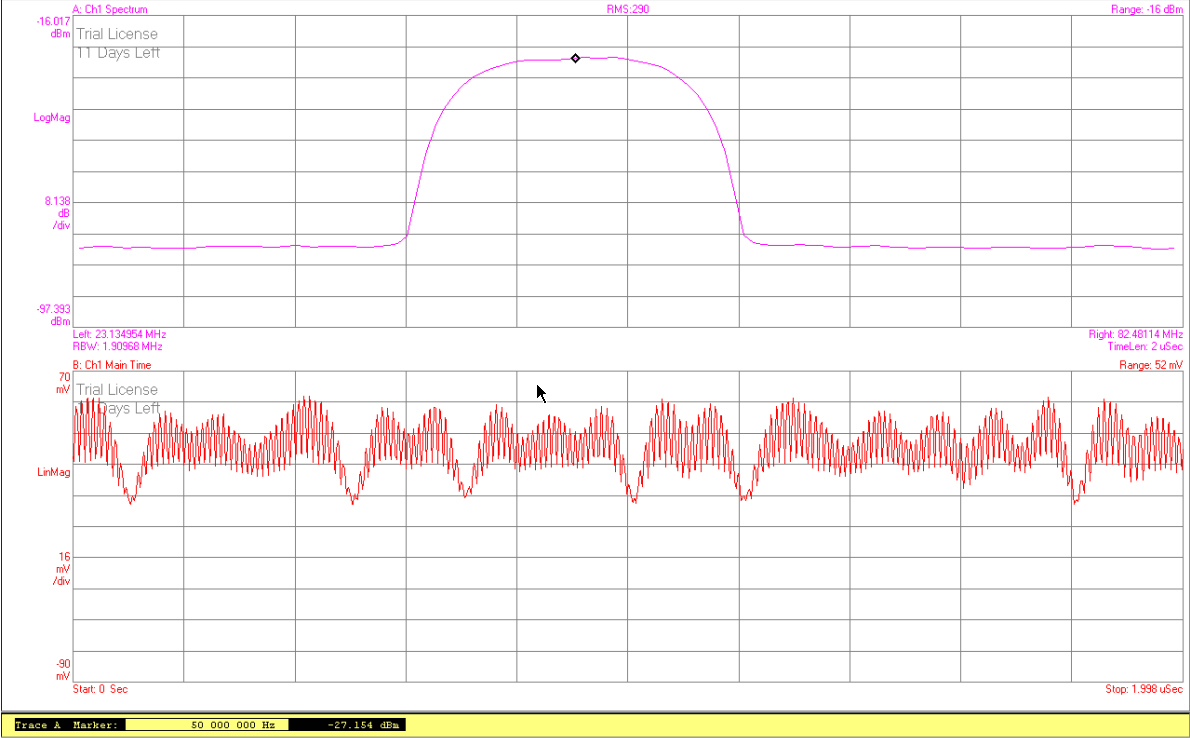
\includegraphics[width=\textwidth]{figures/Aufgabe1_QPSK_avg.jpg} 
\caption{Test}
\end{figure}

\begin{figure}[H]
\centering
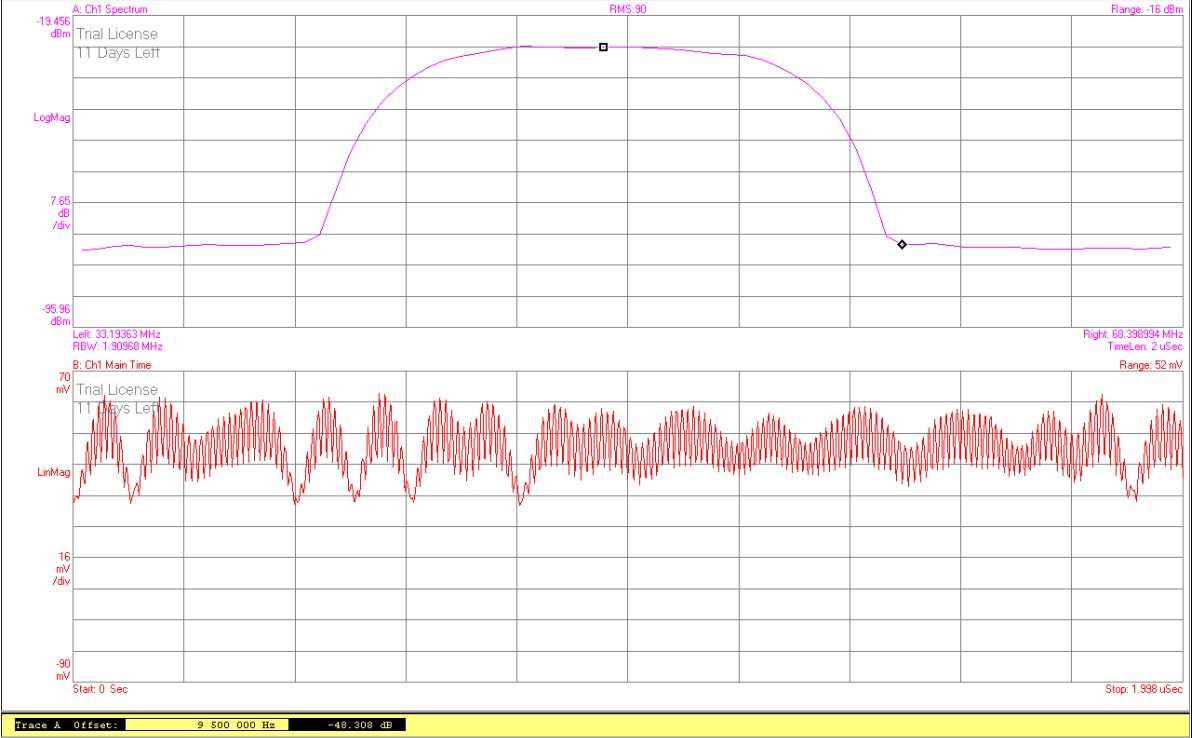
\includegraphics[width=\textwidth]{figures/Aufgabe1_QPSK_B.jpg} 
\caption{Test}
\end{figure}

\begin{figure}[H]
\centering
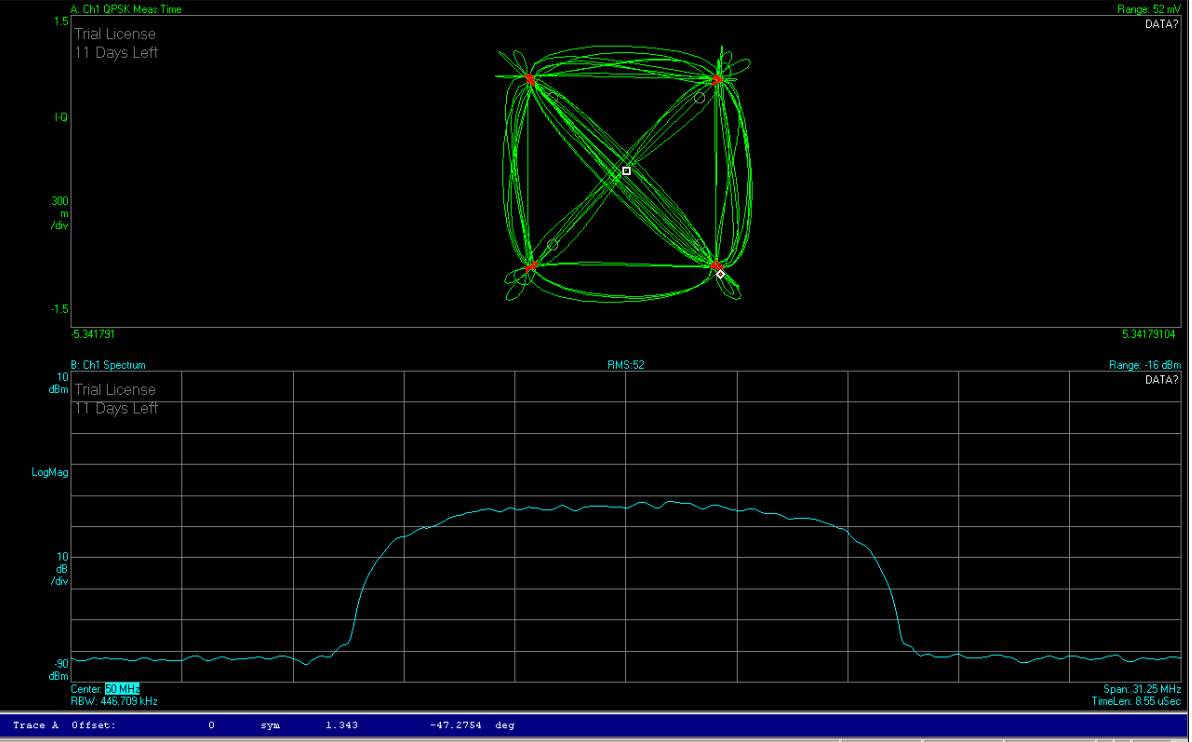
\includegraphics[width=\textwidth]{figures/Aufgabe1_QPSK_demod.jpg} 
\caption{Test}
\end{figure}

\begin{figure}[H]
\centering
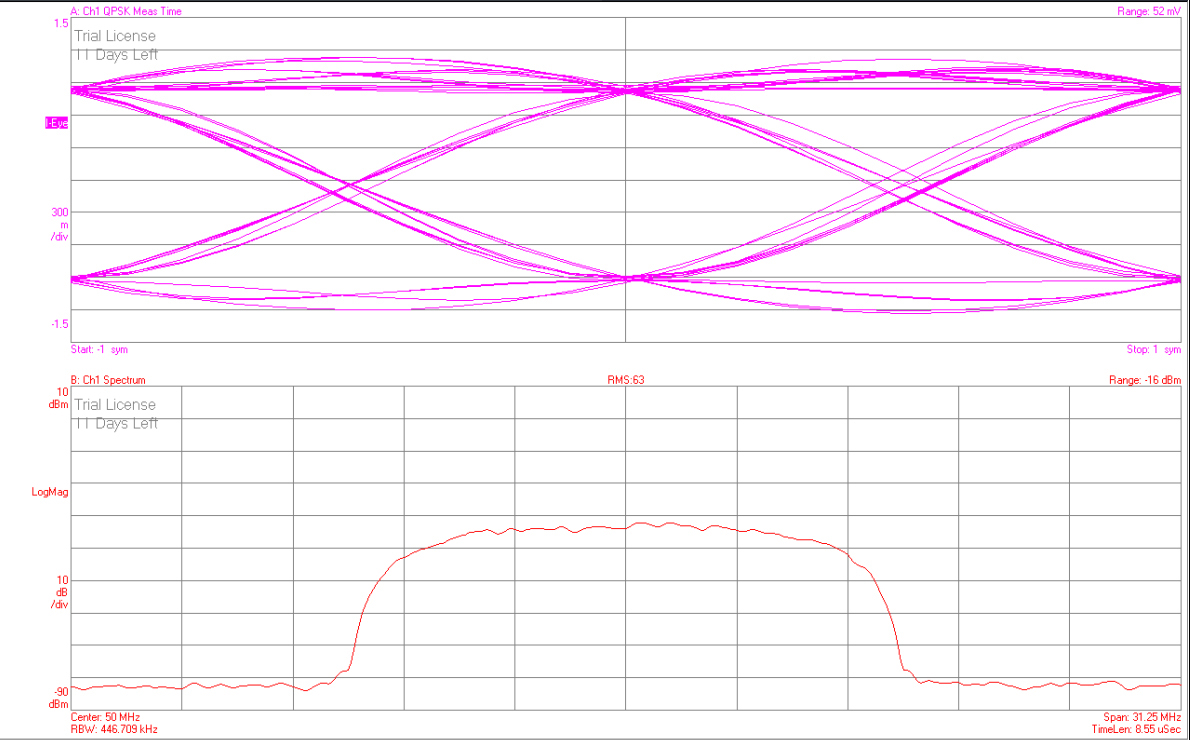
\includegraphics[width=\textwidth]{figures/Aufgabe1_QPSK_demod_i_eye.jpg} 
\caption{Test}
\end{figure}

\begin{figure}[H]
\centering
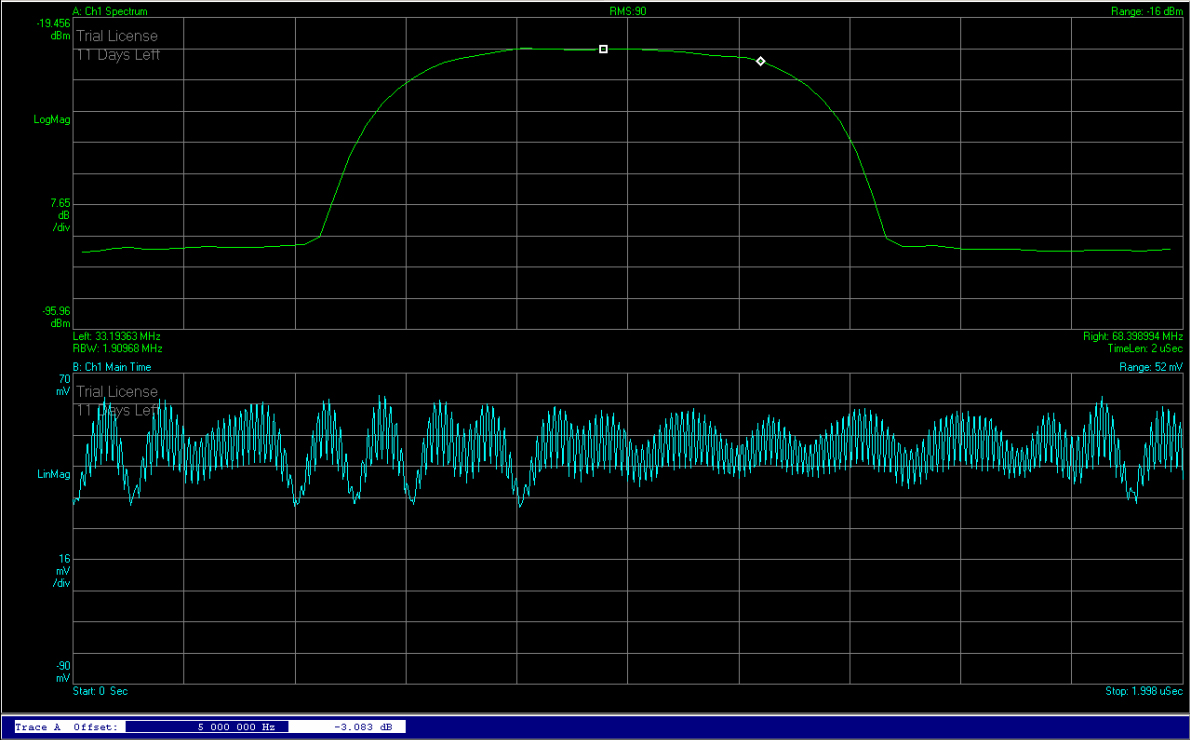
\includegraphics[width=\textwidth]{figures/Aufgabe1_QPSK_fs.jpg} 
\caption{Test}
\end{figure}

\subsection{Diskussion}



\pagebreak



\section{Kanalverzerrungen / Equalizer}
\subsection{Aufgabenstellung}
Ein mittels 16-QAM moduliertes breitbandiges Signal wird über einen nicht-idealen Kanal mit Bandbegrenzung übertragen. Es soll die entstandenen Verzerrungen mit einem Equalizer entfernt werden. Weiters soll die Übertragunsfunktion des Kanals dargestellt werden. 
\begin{itemize}
\item Beurteilen Sie die Verzerrungen anhand des Spektrums.
\item Versuchen Sie, das verzerrte 16-QAM-Signal zu demodulieren. Stellen Sie Augen- und Konstellationsdiagramm dar. Beurteilen Sie anhand dieser Darstellungen die Signalqualität (beachten Sie auch Kenngrößen wie EVM und MER).
\item Wenden Sie einen Equalizer an, um die Verzerrungen zu beseitigen. Wählen Sie dabei verschiedene Darstellungsmöglichkeiten, mit denen Sie die Verbesserung der Signalqualität belegen können. 
\item Stelle Sie die Übertragungsfunktion des Kanals dar. 
\end{itemize}

\subsection{Messaufbau}
Die Kanalverzerrung wurde hier durch den Spektrum Analyzer verursacht. Die Mittenfrequenz des SA wurde auf die Trägerfrequenz des 16-QAM-Signals gelegt und der angezeigte Frequenzbereich auf Null gesetzt. Der SA durchläuft im Normalbetrieb kontinuierlich den eingestellten Messbereich und transformiert zunächst die jeweils aktuelle Frequenz auf eine Zwischenfrequenz (hier 321.4MHz). Wenn der Bereich wie hier aber auf Null gesetzt wird, erfolgt einfach eine Messung mit einer gewissen Bandbreite um die eingestellte Mittenfrequenz herum. Bei dem verwendeten Spectrum Analyzer beträgt diese Bandbreite 30 MHz. Im Bereich von 30-50MHz treten lineare Verzerrungen auf. Der Spectrum Analyzer besitzt einen speziellen Ausgang, an welchem das auf die Zwischenfrequenz transformierte Signal abgegriffen werden kann. 
\begin{figure}[H]
\centering
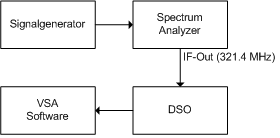
\includegraphics[scale = 1]{figures/uebung2_schaltung.png} 
\caption{Messaufbau für Kanalverzerrung}
\end{figure}
\subsection{Tabellen}
Es waren keine Tabellen aufzunehmen. 
\subsection{Formeln}

\subsection{Berechnungsbeispiele}

\subsection{Diagramme}
\begin{figure}[H]
\centering
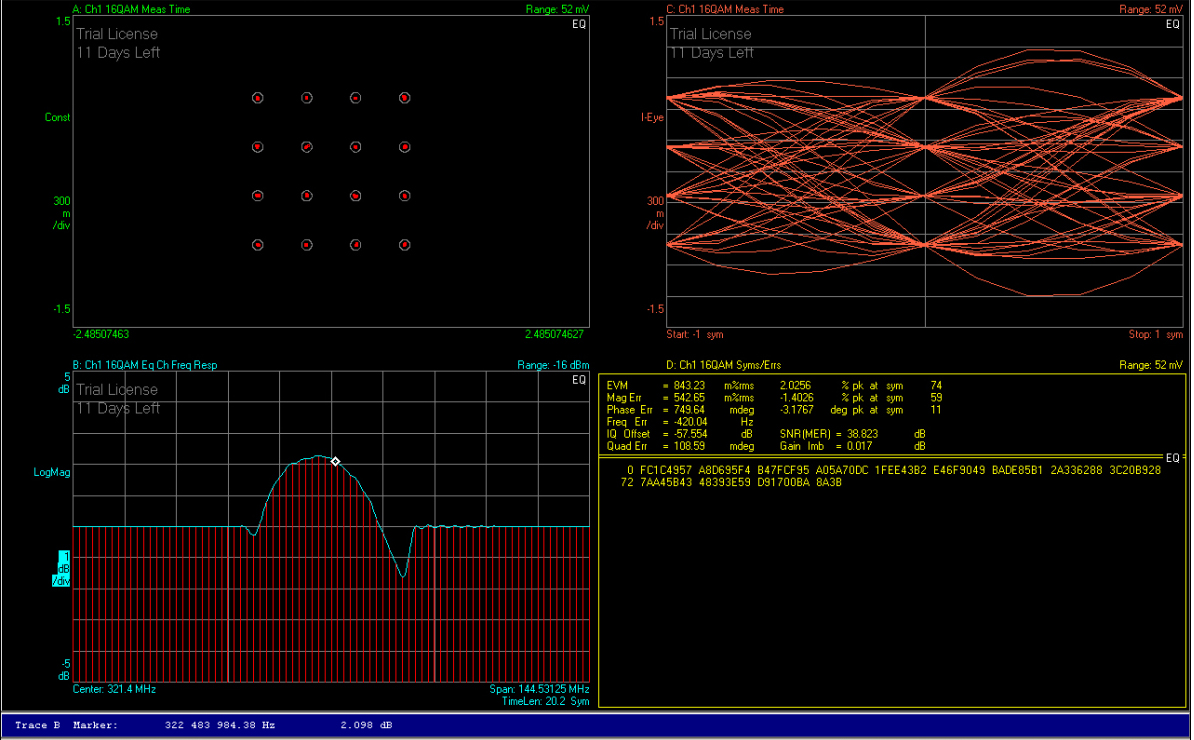
\includegraphics[width=\textwidth]{figures/Aufgabe2_16QAM.jpg} 
\caption{Test}
\end{figure}

\begin{figure}[H]
\centering
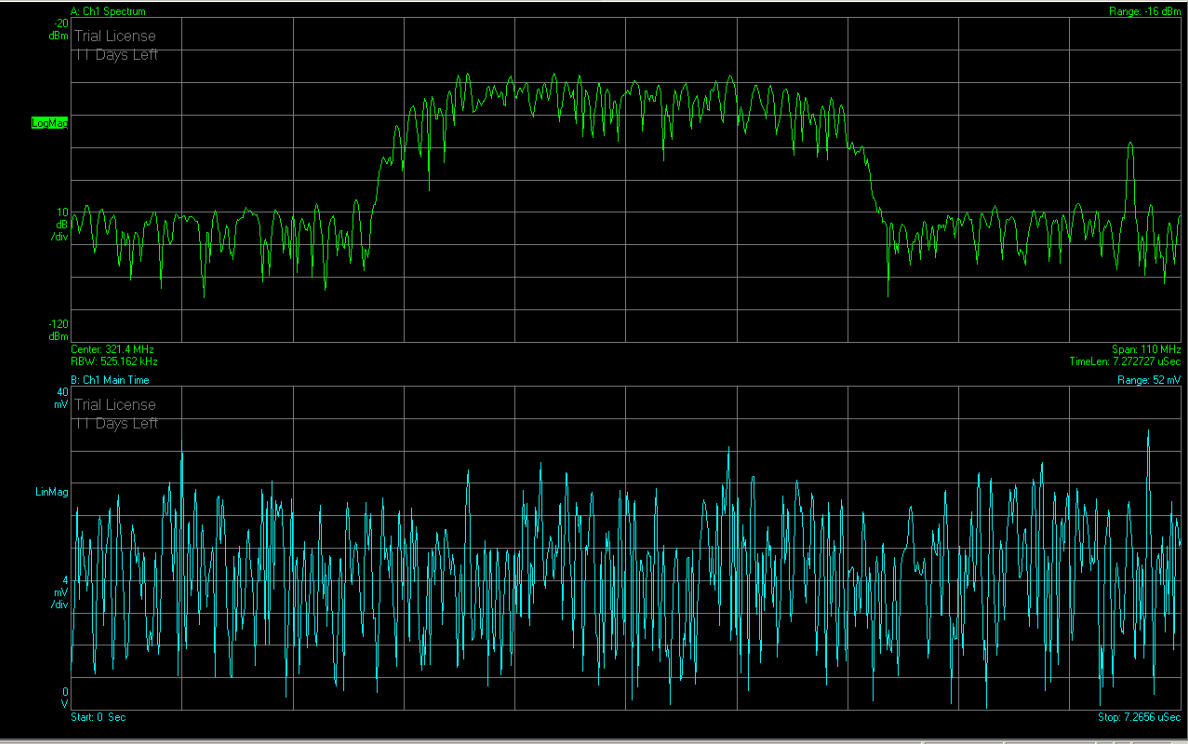
\includegraphics[width=\textwidth]{figures/Aufgabe2_16QAM_1.jpg} 
\caption{Test}
\end{figure}

\begin{figure}[H]
\centering
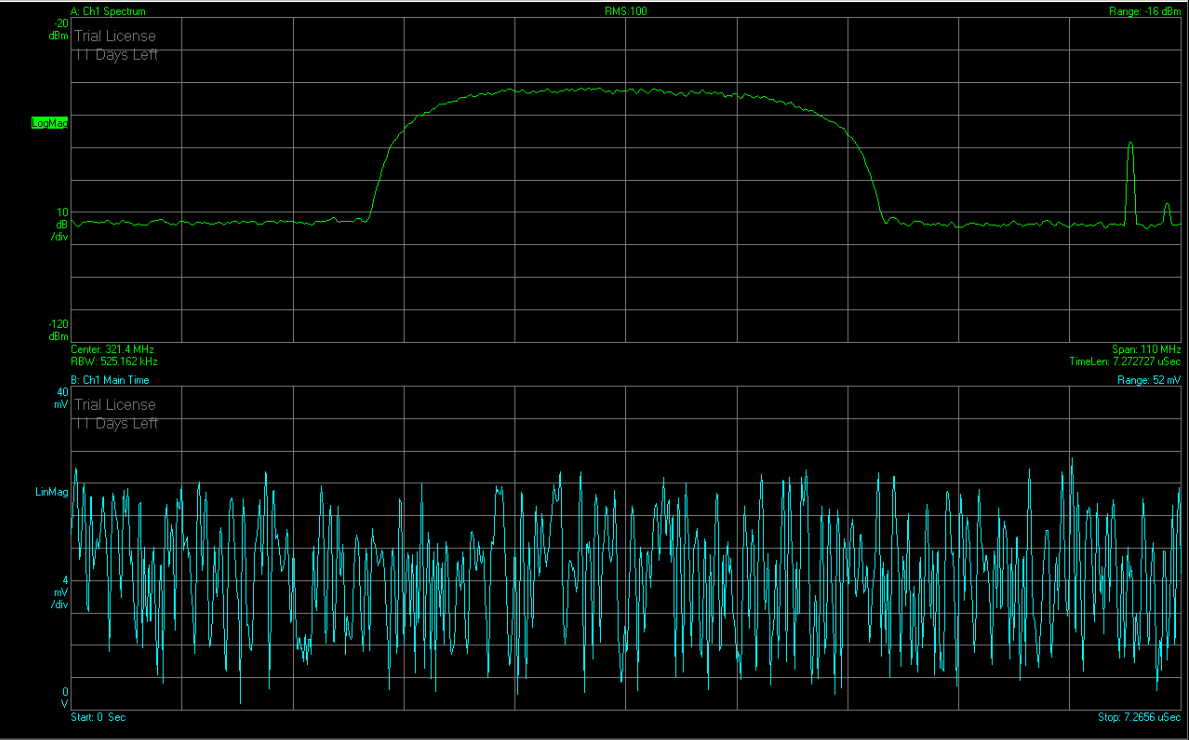
\includegraphics[width=\textwidth]{figures/Aufgabe2_16QAM_avg.jpg} 
\caption{Test}
\end{figure}

\begin{figure}[H]
\centering
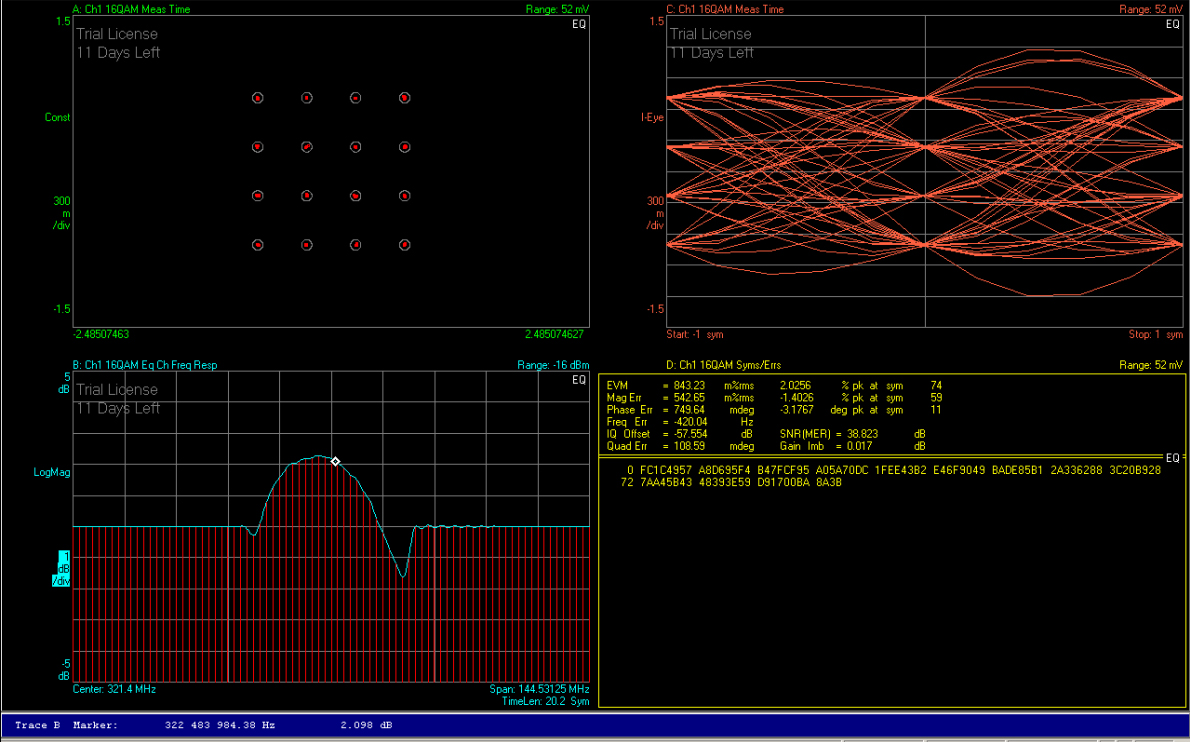
\includegraphics[width=\textwidth]{figures/Aufgabe2_16QAM_demod_equal.jpg} 
\caption{Test}
\end{figure}


\subsection{Diskussion}



\pagebreak



\section{Vergleich digitaler Phasenmodulationsverfahren}
\subsection{Aufgabenstellung}
Gegeben ist eine Reihe von Signalen, welche mit unterschiedlichen digitalen Phasenmodulationsverfahren moduliert wurden (QPSK, $\pi/4$-DQPSK, OQPSK, MSK und GMSK). Da es sich um Phasenmodulationsverfahren handelt, sollte die Hüllkurve dieser Signale idealerweise konstant sein. Speziell bei QPSK gibt es aber mitunter starke Einbrüche in der Hüllkurve. Sie sollen nun eine Reihe von Modualtionsverfahren auf ihre Eigenschaften untersuchen. 
\begin{itemize}
\item Demodulieren Sie die Signale und beurteilen Sie die Übergänge zwischen den Symbolen. Diskutieren Sie den Einfluss dieser Übergänge auf die Hüllkurve. 
\item Stellen Sie den Phasenverlauf dar und diskutieren Sie diesen.
\item Finden Sie einen alternativen Weg, Aussagen über die Hüllkurvenschwankungen treffen zu können.
\end{itemize}


\subsection{Tabellen}
Es waren keine Tabellen aufzunehmen. 
\subsection{Formeln}

\subsection{Berechnungsbeispiele}

\subsection{Diagramme}
\begin{figure}[H]
\centering
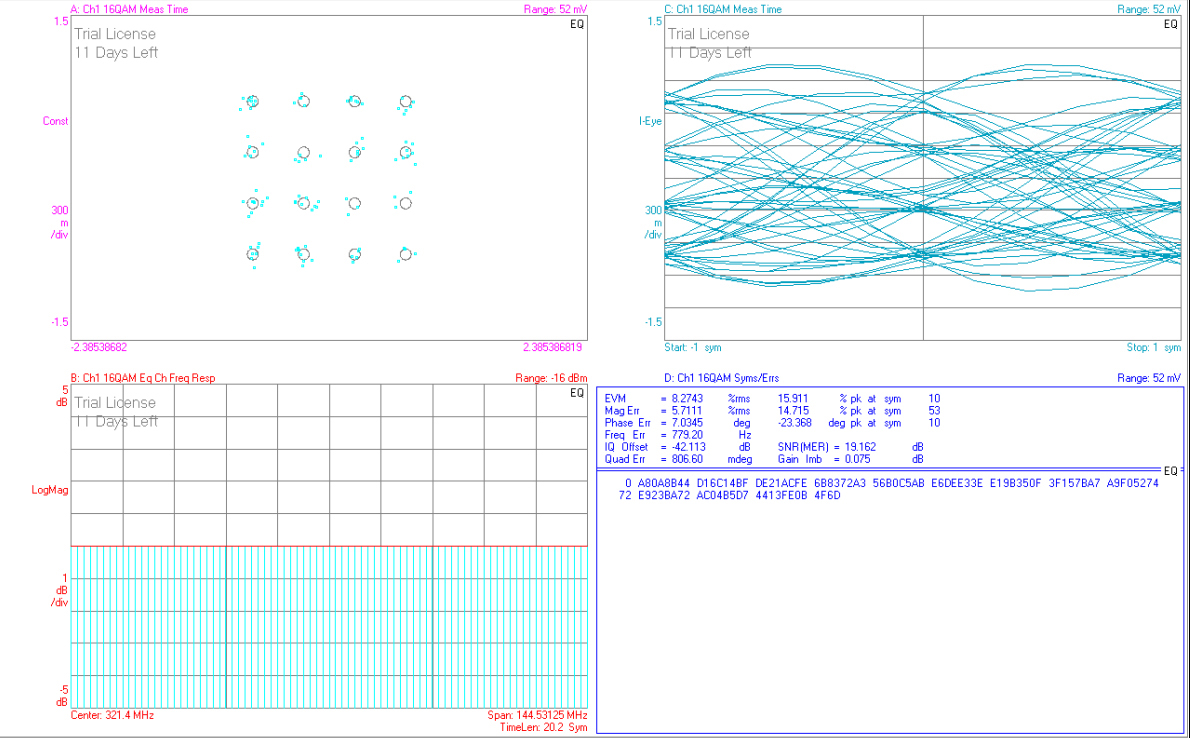
\includegraphics[width=\textwidth]{figures/Aufgabe3_16QAM_demod.jpg} 
\caption{Test}
\end{figure}

\begin{figure}[H]
\centering
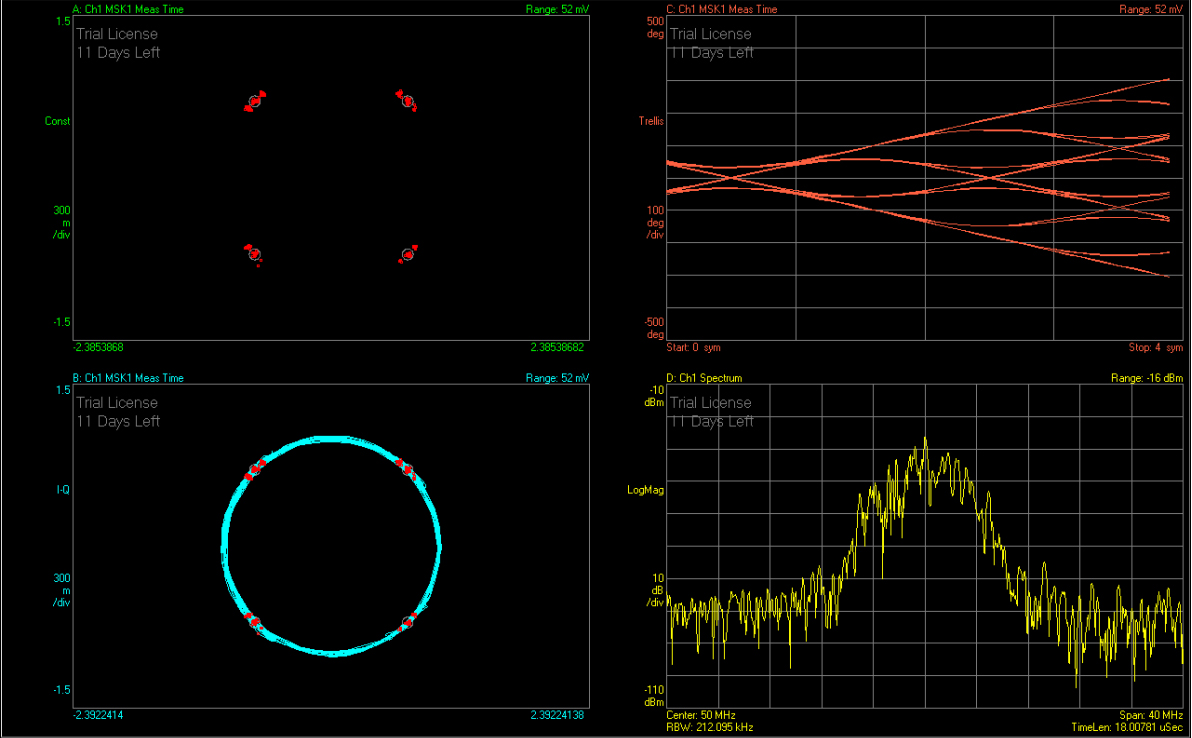
\includegraphics[width=\textwidth]{figures/Aufgabe3_GMSK.jpg} 
\caption{Test}
\end{figure}

\begin{figure}[H]
\centering
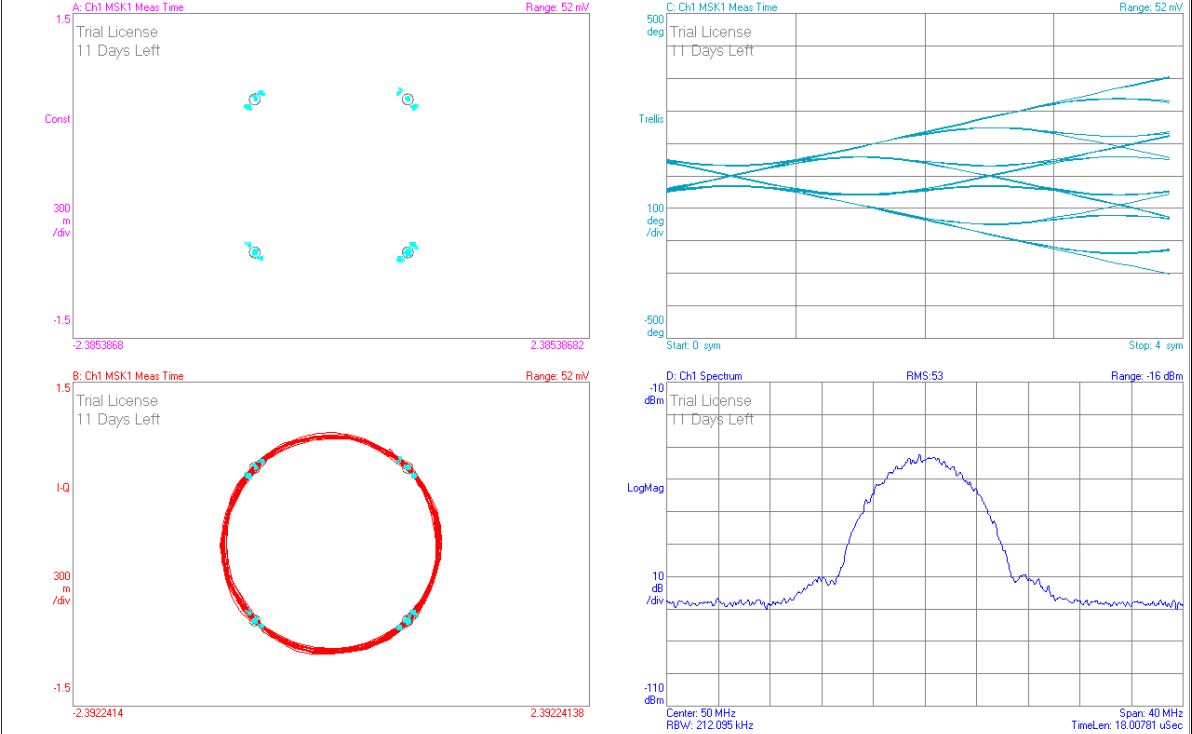
\includegraphics[width=\textwidth]{figures/Aufgabe3_GMSK_avg.jpg} 
\caption{Test}
\end{figure}

\begin{figure}[H]
\centering
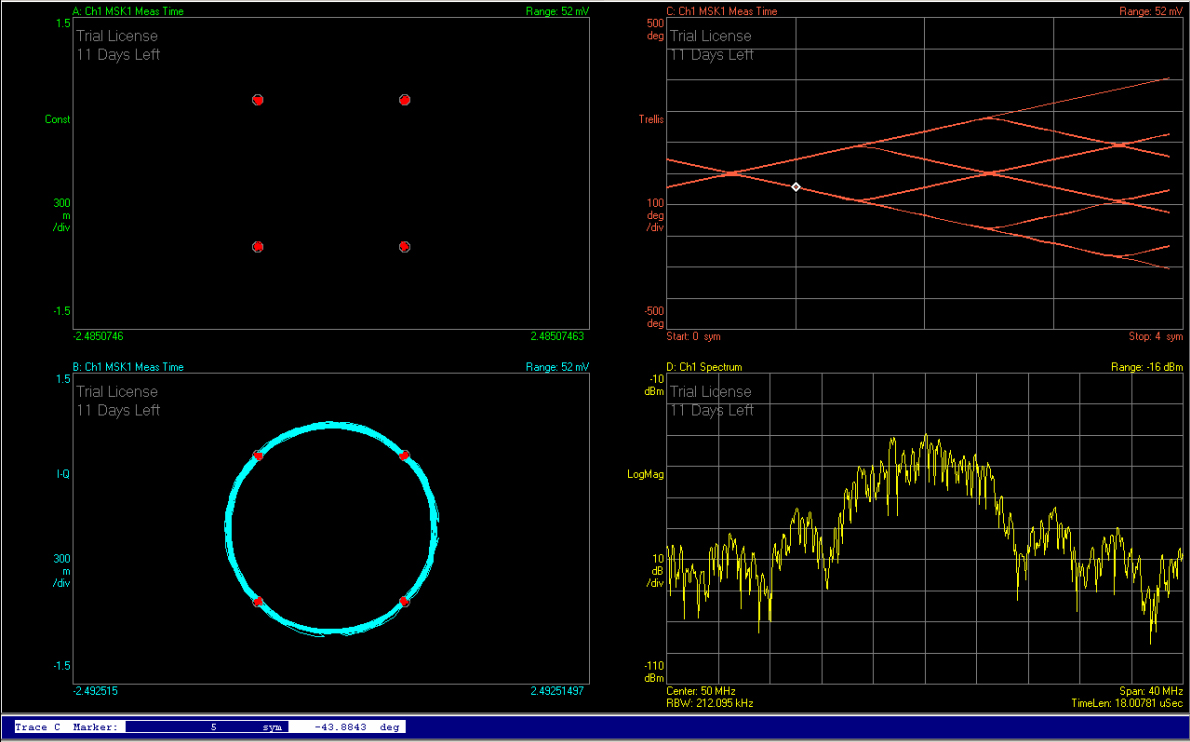
\includegraphics[width=\textwidth]{figures/Aufgabe3_MSK.jpg} 
\caption{Test}
\end{figure}

\begin{figure}[H]
\centering
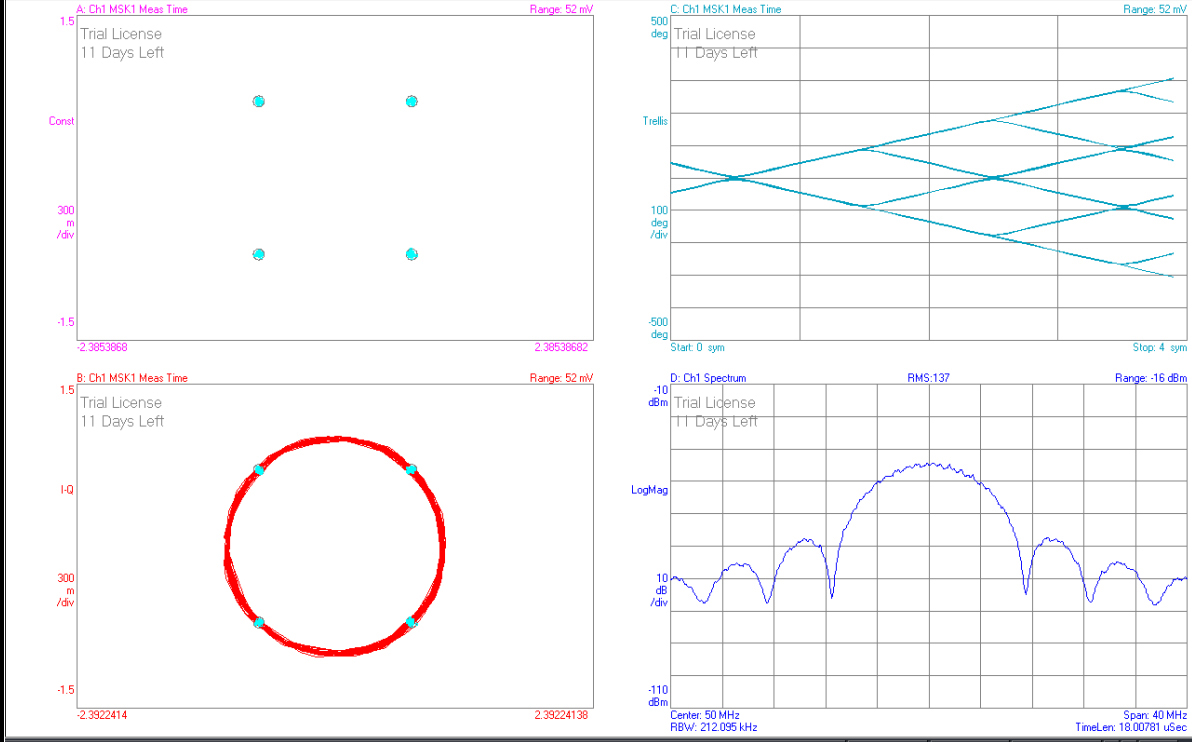
\includegraphics[width=\textwidth]{figures/Aufgabe3_MSK_avg.jpg} 
\caption{Test}
\end{figure}

\begin{figure}[H]
\centering
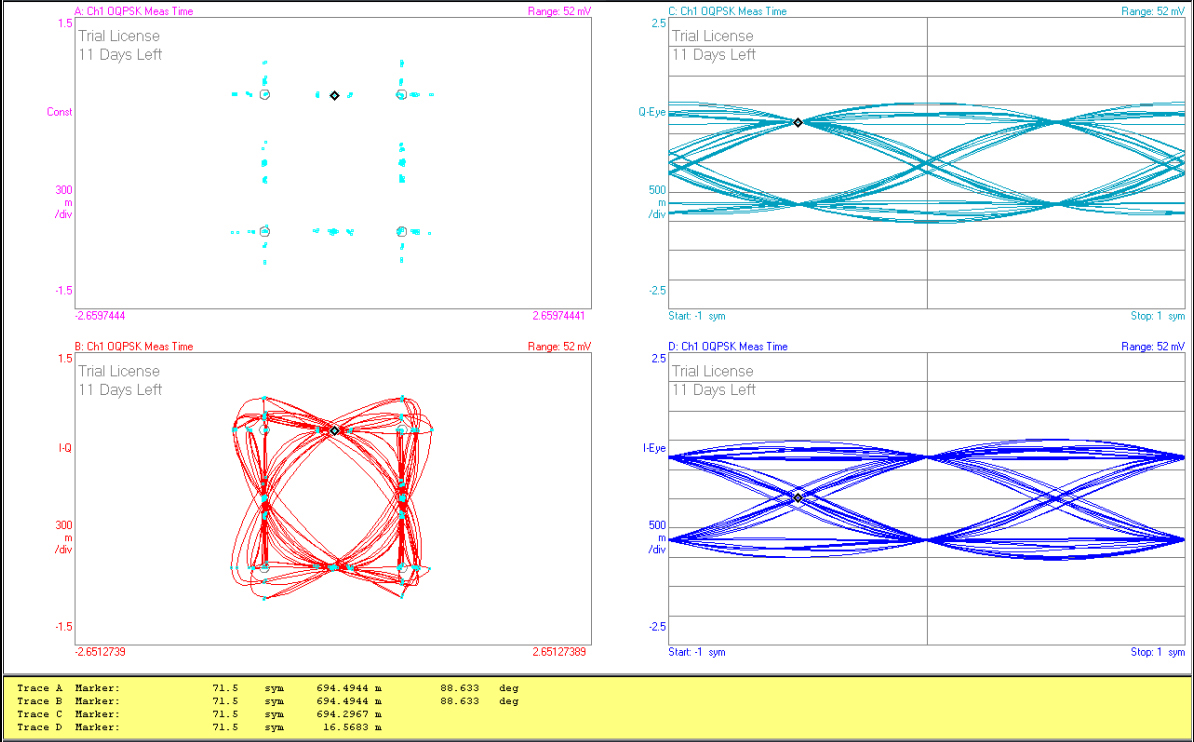
\includegraphics[width=\textwidth]{figures/Aufgabe3_OQPSK.jpg} 
\caption{Test}
\end{figure}

\begin{figure}[H]
\centering
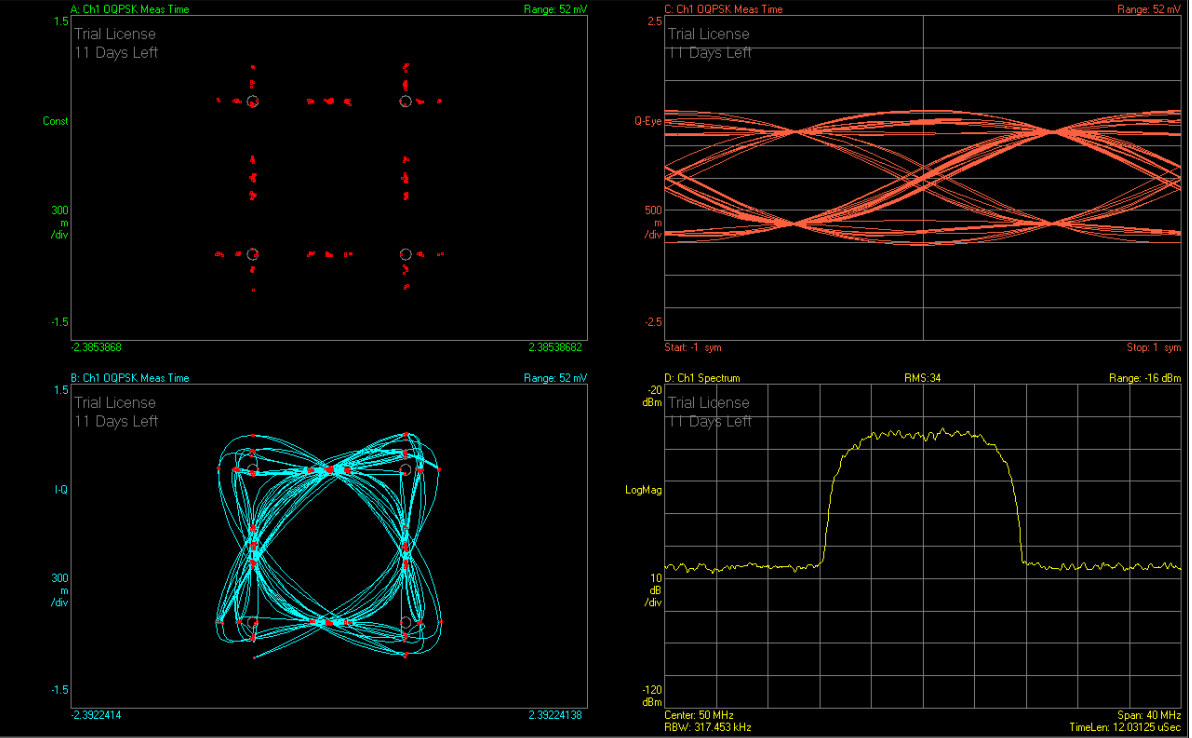
\includegraphics[width=\textwidth]{figures/Aufgabe3_OQPSK_avg.jpg} 
\caption{Test}
\end{figure}

\begin{figure}[H]
\centering
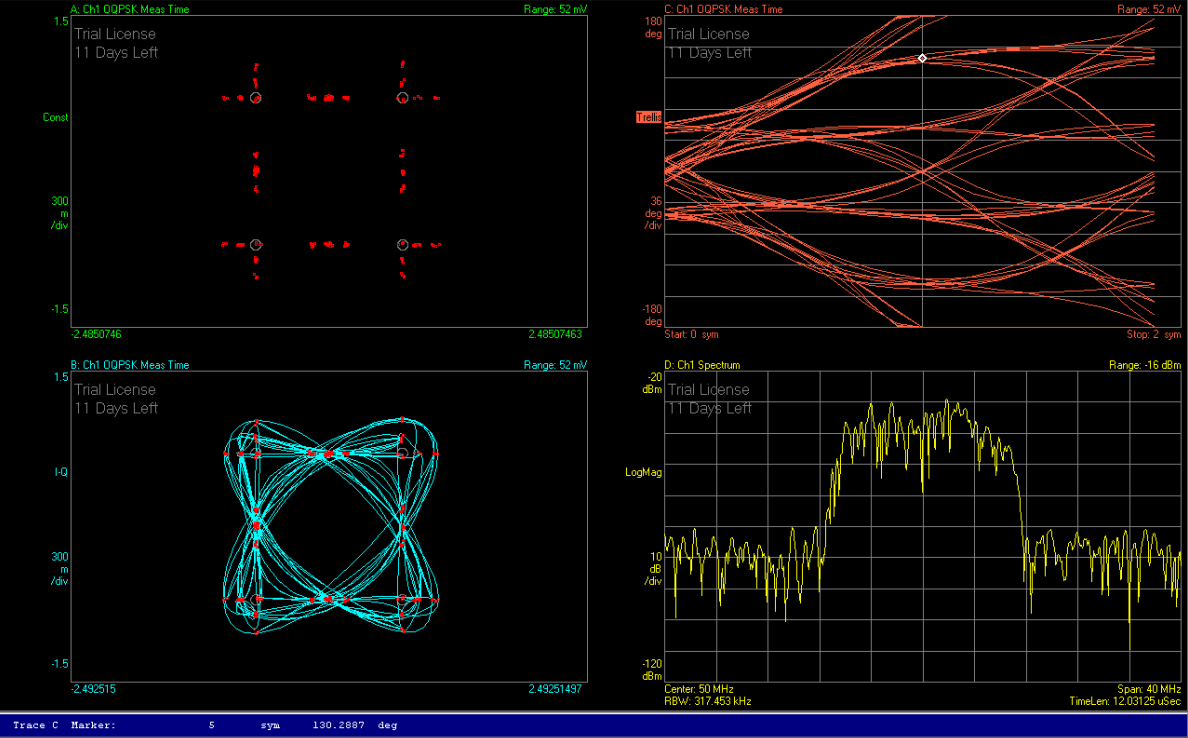
\includegraphics[width=\textwidth]{figures/Aufgabe3_OQPSK_phase.jpg} 
\caption{Test}
\end{figure}

\begin{figure}[H]
\centering
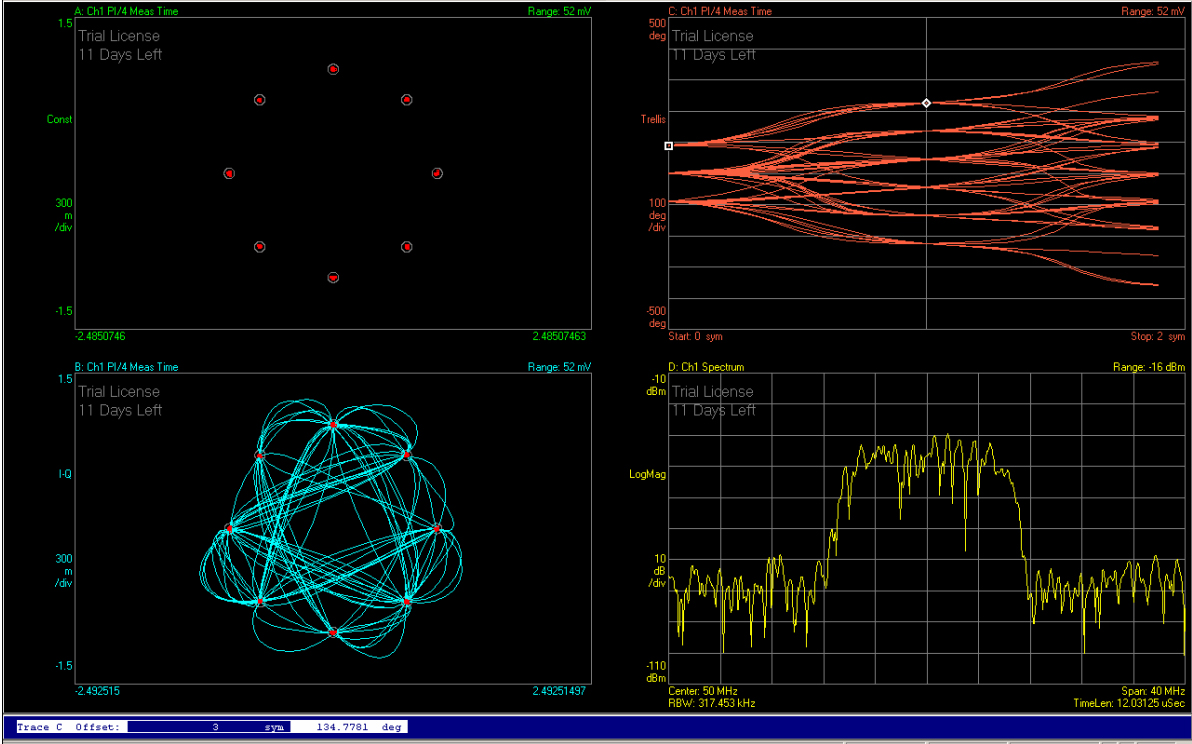
\includegraphics[width=\textwidth]{figures/Aufgabe3_pi4DQPSK.jpg} 
\caption{Test}
\end{figure}

\begin{figure}[H]
\centering
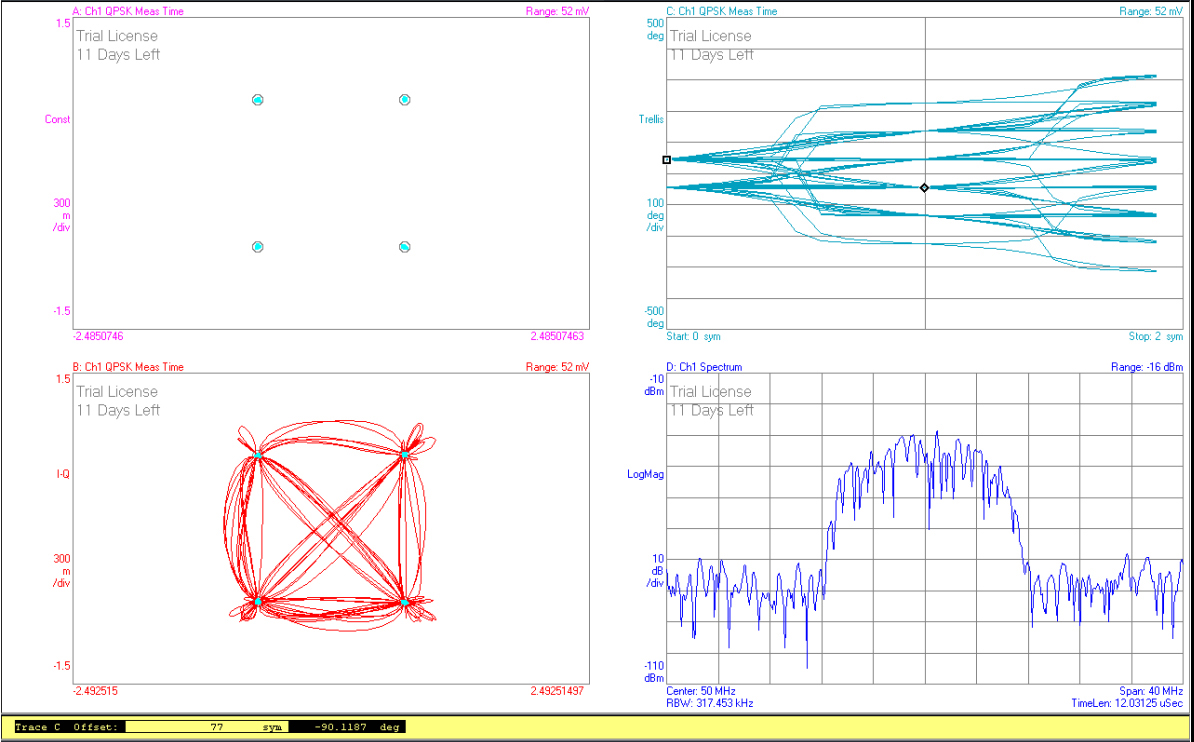
\includegraphics[width=\textwidth]{figures/Aufgabe3_QPSK.jpg} 
\caption{Test}
\end{figure}


\subsection{Diskussion}



\pagebreak



\section{GSM}
\subsection{Aufgabenstellung}
Gegeben ist eine 65ms lange Aufzeichnung aus dem Frequenzbereich von 930-960MHz (oberer Bereich des Downlinks bei GSM 900). Sie sollen in diesem Bereich verschiedene GSM-Kanäle beobachten und ein möglichst starkes Signal demodulieren. Hierzu müssen Sie aufgrund des geringen SNR auf eine genaue Einstellung des Demodulators und des verwendeten Messbereichs achten. 
\begin{itemize}
\item Visualisieren Sie den gegebenen Frequenzbereich mittels Spektrogramm. Suchen Sie einen Kanal, welcher Ihnen zur Untersuchung geeignet erscheint.
\item Versuchen Sie, im Zeitbereich einen Burst zu finden. Versuchen Sie, die GSM Framestruktur zu visualisieren.
\item Stellen Sie den digitalen Demodulator auf die Parameter von GSM ein. Stellen Sie Spektrum, Konstellationsdiagramm und Zeitbereich dar. Diskutieren Sie auch den Phasenverlauf. 
\item Diskutieren Sie die im Skriptum angeführten Parameter von GSM anhand von Spektrum, Spektrogramm, Zeitbereich und digitalem Demodulator. 
\end{itemize}

\subsection{Messaufbau}
Der Messaufbau ähnelt dem von Übung 2, wobei das Signal hier aber nicht generiert, sondern über eine Antenne empfangen wurde. Das wiederum auf $321.4$MHz transformierte Signal wird dem Oszilloskop zur Digitalisierung zugeführt. 
\subsection{Tabellen}
Es waren keine Tabellen aufzunehmen. 
\subsection{Formeln}

\subsection{Berechnungsbeispiele}

\subsection{Diagramme}
\begin{figure}[H]
\centering
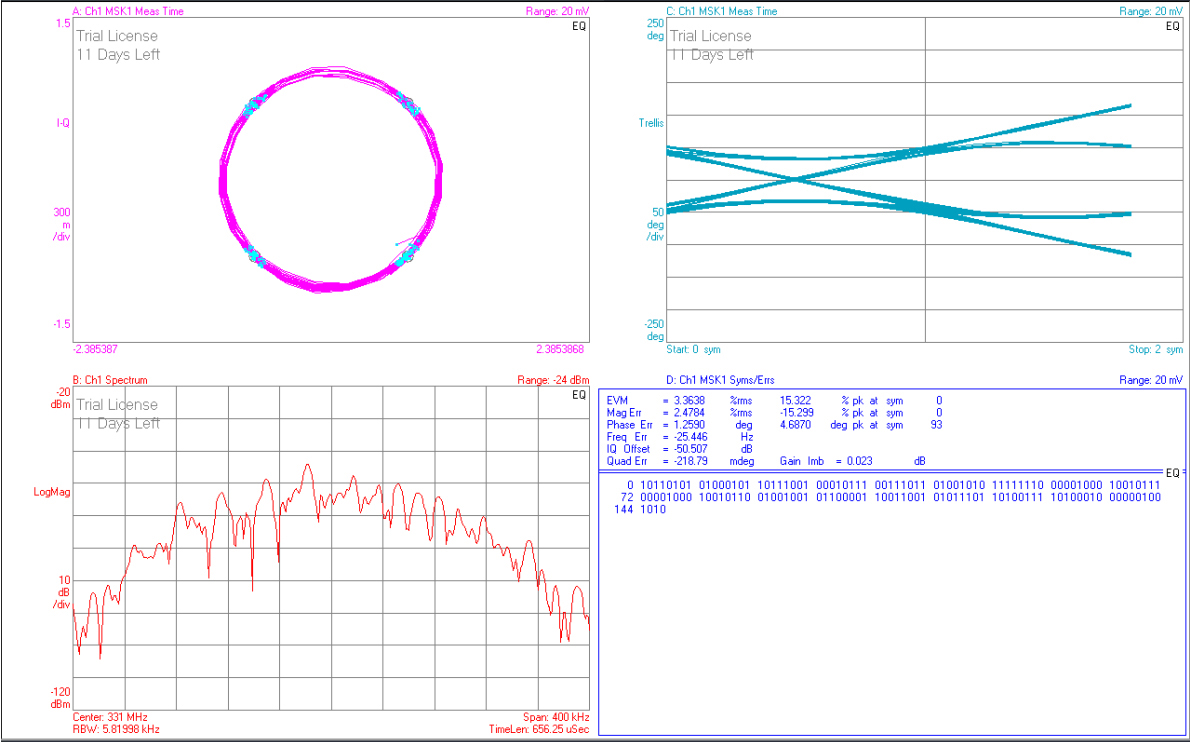
\includegraphics[width=\textwidth]{figures/Aufgabe4_demod.jpg} 
\caption{Test}
\end{figure}

\begin{figure}[H]
\centering
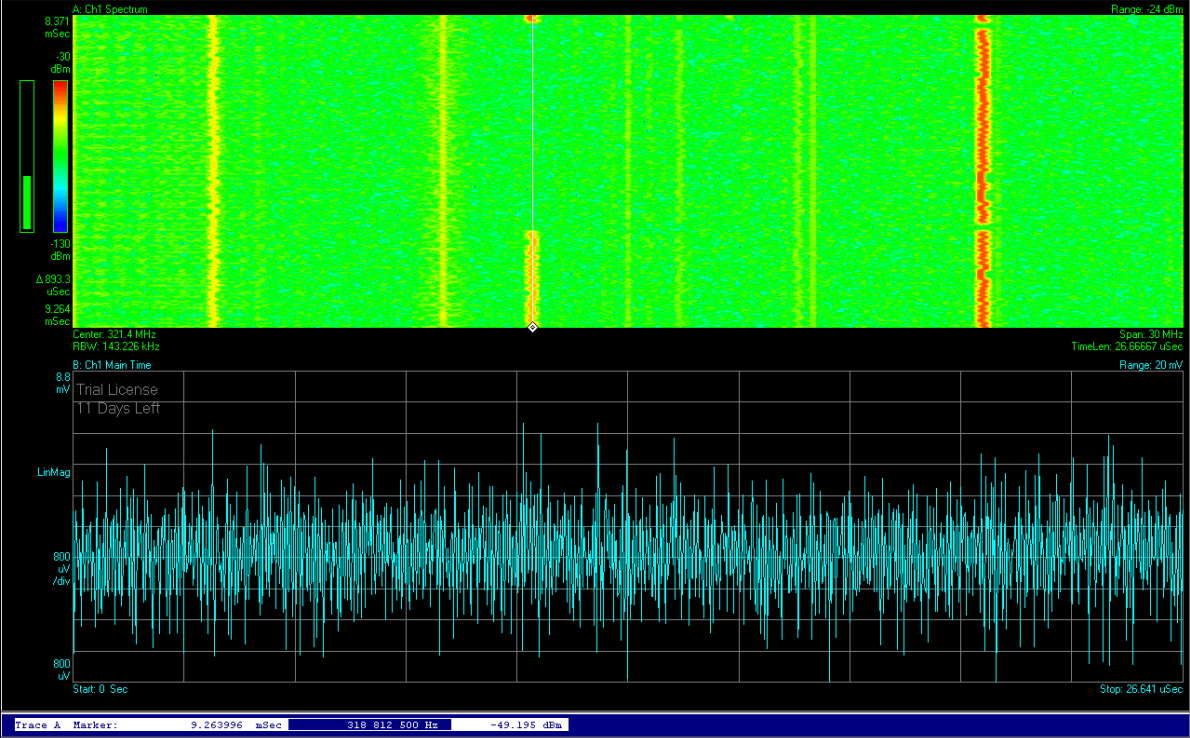
\includegraphics[width=\textwidth]{figures/Aufgabe4_Spektrogramm.jpg} 
\caption{Test}
\end{figure}




\subsection{Diskussion}


 



   
\end{document}